\section{Die Brownsche Bewegung}

Oft wird die Brownsche Bewegung (oder auch Wiener Prozess) axiomatisch definiert. In dieser Arbeit werden 
direkt kumulative Summen von Normalverteilungen betrachtet. Zuerst wird eine vereinfachte Darstellung des Prozesses eingeführt, 
die diskrete Brownsche Bewegung. Die Argumentation folgt der Darstellung von Behrends \cite{behrends} (2013, Kap. 5).

\subsection{Die diskrete Brownsche Bewegung}

\begin{defi}[Diskrete Brownsche Bewegung]
Die elementare Brownsche Bewegung sei ein stochastischer Prozess, 
der aus einer Folge von Zufallsvariablen $\xi_n, n \in \Bbb N_0$ besteht, wobei
$$\xi_n = \sum_{i=1}^n \eta_i, \quad \eta_i \sim \mathcal N(0,1).$$
Die Zufallsvariablen $\eta_i$ sind unabhängig und identisch verteilt.
Nun wird eine stetige Zeitentwicklung durch lineare Interpolation eingeführt:
$$b^{(1)}(t) := \xi_{\lfloor t \rfloor} + (t - \lfloor t \rfloor)(\xi_{\lfloor t \rfloor + 1} - \xi_{\lfloor t \rfloor}), \quad t \geq 0.$$
Die Funktion $b^{(1)}(t)$ wird diskrete Brownsche Bewegung erster Ordnung genannt.
Der Name rührt daher, dass in eine Zeiteinheit genau eine Normalverteilung einbezogen wird.
Im Allgemeinen wird die diskrete Brownsche Bewegung $b^{(N)}(t)$ $N$-ter Ordnung definiert als
$$b^{(N)}(t) := \frac{1}{\sqrt{N}} \left ( \xi_{\lfloor Nt \rfloor} + (Nt - \lfloor Nt \rfloor)(\xi_{\lfloor Nt \rfloor + 1} - \xi_{\lfloor Nt \rfloor}) \right ), \quad t \geq 0.$$
Hierbei werden in eine Zeiteinheit $N$ Normalverteilungen einbezogen. Der Faktor $1/\sqrt{N}$ dient dazu, die Varianzen der Normalverteilungen zu normieren.

\end{defi}

\begin{bsp}[Visualisierung der diskreten Brownschen Bewegung]
Das folgende R-Programm (Ausschnitt) generiert eine diskrete Brownsche Bewegung $N$-ter Ordnung.

\begin{lstlisting}
  n_points <- N * T_max
  eta <- rnorm(n_points, mean=0, sd=1)
  xi <- c(0, cumsum(eta))
  t_grid <- seq(0, T_max, length.out=steps)
  k <- floor(N * t_grid)
  frac <- N * t_grid - k
  vals <- xi[k+1] + frac * (xi[k+2] - xi[k+1])
  vals <- vals / sqrt(N)
\end{lstlisting}
Für verschiedene Werte von $N$ ergeben sich die folgenden Grafiken:

\begin{figure}[H]
    \centering
    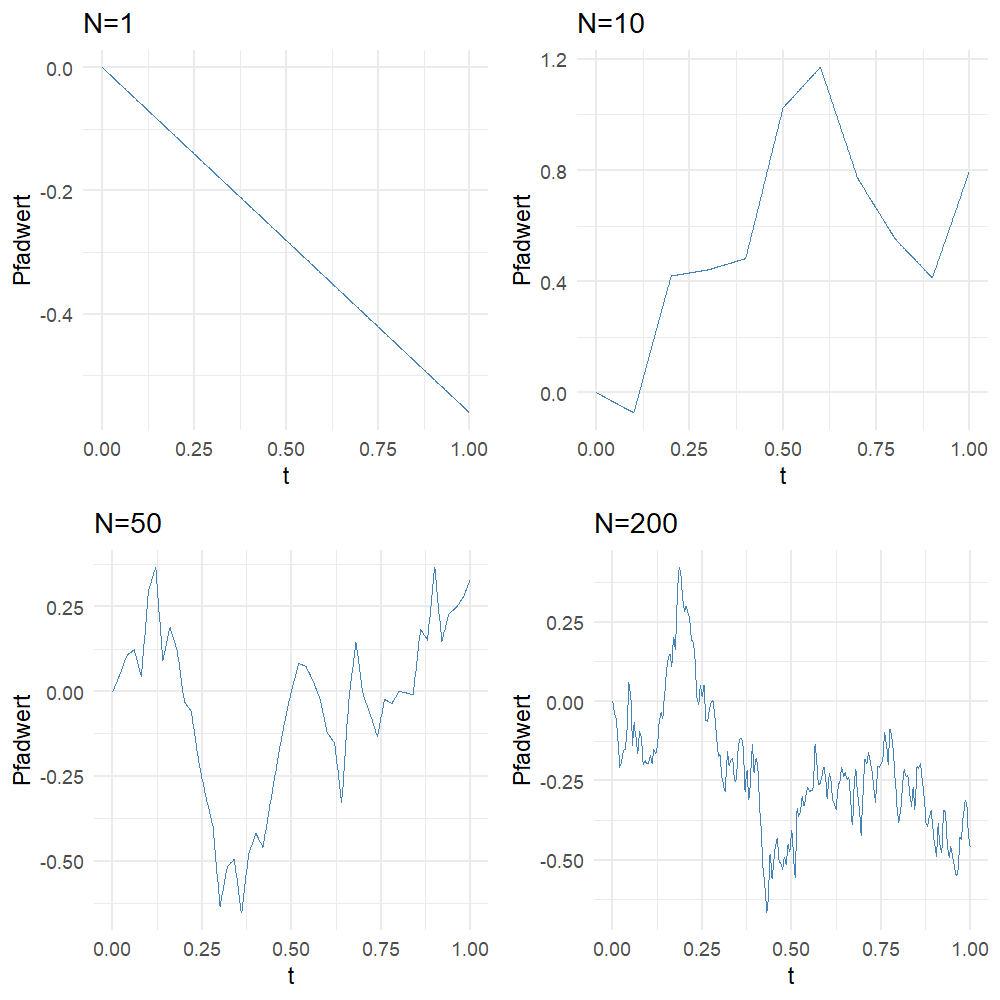
\includegraphics[width=0.9\textwidth]{images/disrete_bb.png}
    \caption{Diskrete Brownsche Bewegung erster, zehnter, fünfzigster und zweihundertster Ordnung}
    \label{fig:brownian}
\end{figure}

\end{bsp}

\begin{lemma}[Erwartungswert der diskreten Brownschen Bewegung]
Es gilt
$$
E(b^{(N)}(t)) = 0.
$$
\textit{Beweis}.
Da $b^{(N)}(t)$ eine lineare Kombination von zentrierten Normalverteilungen ist, gilt
$$
E(b^{(N)}(t)) = \frac{1}{\sqrt{N}} \left( E(\xi_{\lfloor Nt \rfloor}) + (Nt - \lfloor Nt \rfloor) E(\xi_{\lfloor Nt \rfloor + 1} - \xi_{\lfloor Nt \rfloor}) \right).
$$
Da $E(\xi_n) = 0$ für alle $n$ und $E(\xi_{n+1} - \xi_n) = E(\eta_{n+1}) = 0$, folgt
$$
E(b^{(N)}(t)) = 0.
$$
\qed
\end{lemma}

\begin{lemma}[Varianz der diskreten Brownschen Bewegung]
Es gilt
$$
V(b^{(N)}(t)) = \frac{\lfloor Nt \rfloor}{N} + \frac{(Nt - \lfloor Nt \rfloor)^2}{N}.
$$
\textit{Beweis}. Aus der Unabhängigkeit der Inkremente folgt
$$
\begin{aligned}
V(b^{(N)}(t)) &= \frac{1}{N} \left ( V(\xi_{\lfloor Nt \rfloor}) + (Nt - \lfloor Nt \rfloor)^2 \cdot V(\xi_{\lfloor Nt \rfloor + 1} - \xi_{\lfloor Nt \rfloor}) \right ) 
\\ &= \frac{1}{N} (\lfloor Nt \rfloor + (Nt - \lfloor Nt \rfloor)^2)  
\\ &= \frac{\lfloor Nt \rfloor}{N} + \frac{(Nt - \lfloor Nt \rfloor)^2}{N}.
\end{aligned}
$$
\qed
\\
Im Grenzübergang $N \to \infty$ konvergiert $\frac{\lfloor Nt \rfloor}{N} \to t$ und $\frac{(Nt - \lfloor Nt \rfloor)^2}{N} \to 0$.
\end{lemma}

\subsection{Die Brownsche Bewegung als Grenzprozess}
Nun wird der Grenzprozess $N \to \infty$ betrachtet. Intuitiv wird die Zeit immer feiner aufgelöst,
und es werden immer mehr Normalverteilungen in eine Zeiteinheit einbezogen. Vorerst ist jedoch unklar, 
ob der Grenzprozess überhaupt existiert. Um die Konvergenz des Prozesses zu zeigen, wird die Verteilungskonvergenz 
untersucht. Konvergenz der einzelnen Zeitpunkte (oder endlich-dimensionalen Vektoren) reicht nicht 
für Konvergenz der Prozesse als Funktionen. Daher wird die Konvergenz in 3 Schritten untersucht:
\begin{enumerate}
  \item Verteilungskonvergenz der einzelnen Zeitpunkte
  \item Verteilungskonvergenz von endlich-dimensionalen Vektoren und die Kovarianzen (Hieraus folgt bereits die Selbstähnlichkeit und bedingte Verteilung so wie die Martingal-Eigenschaft)
  \item Stetigkeit der Pfade des Grenzprozesses
\end{enumerate}
Die Verteilungskonvergenz im Funktionenraum $C[0, 1]$ der stetigen Funktionen $f : [0, 1] \to \Bbb R$ wird in dieser Arbeit nicht behandelt.
Diese kann mit dem Satz von Donsker (\cite{henze2022asymptotische}, S. 270) nachgewiesen werden.

\begin{lemma}[Verteilungskonvergenz zu einzelnen Zeitpunkten]
Es existiert ein stochastischer Prozess $W_t, t \geq 0$, so dass für jedes $t$ die Verteilung von $b^{(N)}(t)$ gegen die Verteilung von $W_t$ konvergiert, wenn $N \to \infty$.
\textit{Beweis.}
Da 
$$b^{(N)}(t) = \frac{1}{\sqrt{N}}\big(\xi_k+\alpha(\xi_{k+1}-\xi_k)\big)
=\frac{1}{\sqrt{N}}\big(\xi_k+\alpha\,\eta_{k+1}\big).
$$
ist $b^{(N)}(t)$ eine lineare Kombination von Normalverteilungen, und daher widerum 
normalverteilt. Erwartungswert und Varianz wurden bereits berechnet:
$$
E(b^{(N)}(t)) = 0, \quad V(b^{(N)}(t)) = \sigma_N^2(t) = \frac{1}{N}\big(k+\alpha^2\big),
$$
wobei $k=\lfloor Nt \rfloor$ und $\alpha=Nt-k\in[0,1)$. Damit gilt
$$
b^{(N)}(t) \sim N\left(0,\frac{1}{N}\big(k+\alpha^2\big)\right).
$$
Die Verteilungsfunktion ist gegeben durch
$$
F_N(x)=P\big(b^{(N)}(t)\le x\big)=\Phi\!\left(\frac{x}{\sigma_N(t)}\right),
$$
wobei $\Phi$ die Standardnormalverteilungsfunktion ist. Aus $\sigma_N^2(t)\to t$ folgt $\sigma_N(t)\to \sqrt{t}$ und wegen der Stetigkeit von $\Phi$ daher
$$
F_N(x)=\Phi\!\left(\frac{x}{\sigma_N(t)}\right)\; \xrightarrow[N \to \infty]{\mathrm{pktw}} \;\Phi\!\left(\frac{x}{\sqrt{t}}\right)\quad\text{für alle }x\in\Bbb R.
$$
Dies ist die Verteilungsfunktion von $N(0,t)$. Definiere $W_t :\sim \mathcal N(0,t)$. Somit konvergiert für jedes feste $t$ die Verteilung von $b^{(N)}(t)$ gegen die von $W_t$. 
\qed
\end{lemma}

\begin{satz}[endlich-dimensionale Verteilungskonvergenz und Kovarianzstruktur der Brownschen Bewegung]
Aus der Verteilungskonvergenz der einzelnen Zeitpunkte kann man noch keinen sinnvollen Grenzprozess folgern.
Die Zeitpunkte $W_t$ sind zwar normalverteilt, aber der Prozess könnte trotzdem sprunghaft sein.
Nun wird die Verteilungskonvergenz der endlich-dimensionalen Vektoren gezeigt, beziehungsweise
die Kovarianz der Realisierungen bei benachbarten Zeitpunkten untersucht. Für $t$ und $s$ gilt 
$$
\mathrm{Cov}(W_s, W_t) = \min(s,t).
$$
Sei $0\le t_1\le\cdots\le t_k$ eine Zerlegung. Dann gilt
$$
\big(b^{(N)}(t_1), \dots , b^{(N)}(t_k) \big )\;\xrightarrow[N \to \infty]{\mathrm{d}}\;\big(W_{t_1},\dots,W_{t_k}\big).
$$
\textit{Beweis.}\footnote{angelehnt an Henze, 2023 \cite{henze} S. 225f.}
Für jedes $N$ ist der Vektor $\big(b^{(N)}(t_1),\dots,b^{(N)}(t_k)\big)$ gemeinsam normalverteilt,
denn $b^{(N)}(t)$ ist eine lineare Kombination der i.i.d. Standardnormalen $(\eta_i)$.

Es genügt, Mittelwerte und Kovarianzen zu kontrollieren:
Die Mittelwerte sind Null. Für $s,t\ge0$ mit $k=\lfloor Nt\rfloor$, $\alpha=Nt-k$, 
$\ell=\lfloor Ns\rfloor$, $\beta=Ns-\ell$ gilt mit $\xi_n=\sum_{i=1}^n\eta_i$:
$$
b^{(N)}(t)=\tfrac1{\sqrt N}\big(\xi_k+\alpha\eta_{k+1}\big),\qquad
b^{(N)}(s)=\tfrac1{\sqrt N}\big(\xi_\ell+\beta\eta_{\ell+1}\big).
$$
Unabhängigkeit der $\eta_i$ ($E(\eta_i)=0$, $V(\eta_i)=1$) liefert
$$
\begin{aligned}
\mathrm{Cov}\!\big(b^{(N)}(s),b^{(N)}(t)\big) &= E \left [ b^{(N)}(s) b^{(N)}(t) \right ] - \underbrace{E(b^{(N)}(s)) \cdot b^{(N)}(t)}_{=0}
\\ &= \frac{1}{N} E \left [ (\xi_k + \alpha \eta_{k+1}) (\xi_\ell + \alpha \eta_{\ell+1}) \right ] 
\\ &= \frac{1}{N} \left [ E(\xi_\ell \xi_k) + \alpha E(\xi_\ell \eta_{k+1}) + \beta E(\eta_{\ell + 1} \xi_k) + \alpha \beta E(\eta_{\ell + 1} \eta_{k+1}) \right ]
\end{aligned}
$$
Da die Erwartungswerte der $\eta$s gleich Null sind und die $\eta$s unabhängig sind, können die Terme weiter reduziert werden.
$$
\begin{aligned}
E(\xi_\ell \xi_k) &= \sum_{i=1}^\ell \sum_{j=1}^k E(\eta_i \eta_j) \begin{cases} = E(\eta_i)\cdot E(\eta_j) = 0, \quad &i \neq j \\ = E(\eta_i^2) = 1, \quad &i = j \end{cases}
\\ &= \sum_{i=1}^\ell \sum_{j=1}^k \delta_{i, j} = \min(\ell, k)
\end{aligned}
$$
Analog folgt für die anderen Terme z. B.
$$\alpha E(\xi_\ell \eta_{k+1}) = \alpha \sum_{i=1}^\ell E(\eta_i \eta_{k+1}) = \alpha \mathbf 1_{\{k+1\le \ell\}},$$
und so weiter. Insgesamt ergibt sich
$$
\mathrm{Cov}\!\big(b^{(N)}(s),b^{(N)}(t)\big) = \frac1N\Big(\min(\ell,k)+\alpha\,\mathbf 1_{\{k+1\le \ell\}}+\beta\,\mathbf 1_{\{\ell+1\le k\}}+\alpha\beta\,\mathbf 1_{\{\ell=k\}}\Big)
$$
Im Grenzübergang gilt
$$
\mathrm{Cov}\!\big(b^{(N)}(s),b^{(N)}(t)\big)
=\frac{\min(\ell,k)}{N}+O\!\left(\frac1N\right)\xrightarrow[N\to\infty]{}\min(s,t).
$$
Folglich konvergiert die Kovarianzmatrix der Vektoren gegen 
$\Sigma=(\min(t_i,t_j))_{i,j}$.
Mit der Cramér–Wold-Technik reicht es, lineare Formen zu betrachten. Sei also $a=(a_1,\dots,a_k)^\top\in\Bbb R^k$ und
$$
Y_N:=\sum_{i=1}^k a_i\,b^{(N)}(t_i),\qquad
Y:=\sum_{i=1}^k a_i\,W_{t_i},
$$
wobei
$$
V(Y_N)=\sum_{i,j=1}^k a_i a_j\,\mathrm{Cov}\!\big(b^{(N)}(t_i),b^{(N)}(t_j)\big),
$$
und damit
$$
V(Y_N)\xrightarrow[N\to\infty]{}\sum_{i,j=1}^k a_i a_j\,\min(t_i,t_j)=:\sigma^2(a).
$$
Jedes $Y_N$ ist eine lineare Kombination unabhängiger $\eta_i$. Mit dem Zentralen Grenzwertsatz (von Lindeberg-Feller) wird die Grenzverteilung von $Y_N$ bestimmt.
Da die Summanden zentriert und von endlicher Varianz sind, bleibt die Lindeberg-Bedingung zu zeigen. Zerlege
$$
Y_N=\sum_{i=1}^k a_i b^{(N)}(t_i)=\sum_{j=1}^{M_N} c_{N,j}\,\eta_j,
$$
wobei $M_N=\lfloor Nt_k\rfloor+1$ und die Koeffizienten $c_{N,j}$ aus der Definition von $b^{(N)}(t_i)$ stammen.
Aus der Darstellung folgt, dass $|c_{N,j}|\le C/\sqrt N$ für ein von $N$ unabhängiges $C>0$ gilt: Die Definition
$$
\begin{aligned}
b^{(N)}(t) &\overset{\mathrm{def}}= \frac{1}{\sqrt{N}} \left ( \xi_{\lfloor Nt \rfloor} + (Nt - \lfloor Nt \rfloor)(\xi_{\lfloor Nt \rfloor + 1} - \xi_{\lfloor Nt \rfloor}) \right )
\\ &= \frac{1}{\sqrt{N}} \left ((Nt - \lfloor Nt \rfloor) \cdot \eta_{n+1} + \sum_{i=1}^n \eta_i \right ),\quad n = \lfloor Nt \rfloor
\end{aligned}
$$
liefert
$$
C = k \cdot \max_{i=1, \dots, k} \vert a_i \vert.
$$
Damit erhält man für jedes $\varepsilon>0$
$$
\mathbf 1_{\{|c_{N,j}\eta_j|>\varepsilon\}}
= \mathbf 1_{\{|\eta_j|>\varepsilon / \vert c_{N,j} \vert \}}
\le \mathbf 1_{\{|\eta_j|>\varepsilon\sqrt N/C\}}.
$$
Also
$$
L_N(\varepsilon) = \sum_{j=1}^{M_N} E \left (c_{N,j}^2\eta_j^2\,\mathbf 1_{\{|c_{N,j}\eta_j|>\varepsilon\}} \right )
\le \Big(\sum_{j=1}^{M_N} c_{N,j}^2 \Big) E \left [ \eta_1^2\mathbf 1_{\{|\eta_1|>\varepsilon\sqrt N/C\}} \right ].
$$
Die Summe der Quadrate $\sum_j c_{N,j}^2$ ist beschränkt, da sie die Varianz von $Y_N$ ist und gegen
$\sigma^2(a)$ konvergiert. Andererseits gilt wegen $\eta_1\in L^2$ und $\varepsilon\sqrt N/C \to \infty$
$$
E \left [ \eta_1^2\mathbf 1_{\{|\eta_1|>\varepsilon\sqrt N/C\}} \right ] \xrightarrow[N\to\infty]{}0.
$$
Damit ist die Lindeberg-Bedingung erfüllt und es folgt
$$
Y_N \xrightarrow{d} Y \sim \mathcal N(0,\sigma^2(a)).
$$
Insgesamt konvergiert für jedes $a$ die Verteilung von $a^\top(b^{(N)}(t_1),\dots,b^{(N)}(t_k))$ gegen die von $a^\top(W_{t_1},\dots,W_{t_k})$.
Nach Cramér–Wold folgt die behauptete Verteilungskonvergenz des Vektors. \qed
\end{satz}

\begin{satz}[Selbstähnlichkeit und bedingte Verteilung der Brownschen Bewegung]
Für jedes $c > 0$ gilt
$$
W_{ct}(\omega) \overset{d}{=} \sqrt{c}\, W_t(\omega) \quad \text{für alle } t \ge 0,
$$
für alle $s < t$ gilt
$$
W_t - W_s \sim \mathcal N(0, t-s),
$$
und die bedingte Verteilung von $W_t$ gegeben $W_s$ ist
$$
W_t \mid W_s \sim N\big(W_s, t-s\big).
$$
\textit{Beweis der ersten Behauptung (Selbstähnlichkeit).} \\
Für $t \ge 0$ gilt $W_{ct} \sim \mathcal N(0, ct)$ und $W_t \sim \mathcal N(0, t)$. Somit gilt
$$
\sqrt{c}\, W_t \sim \mathcal N(0, c t).
$$
Da beide Normalverteilungen denselben Mittelwert $0$ und dieselbe Varianz $ct$ haben, folgt
$$
W_{ct} \stackrel{d}{=} \sqrt{c}\, W_t \quad \text{für jedes } t \ge 0.
$$  
\qed  \\
\textit{Beweis der zweiten Behauptung (Inkremente).} \\
Für $s < t$ gilt
$$
W_t - W_s = \lim_{N \to \infty} \big( b^{(N)}(t) - b^{(N)}(s) \big),
$$
wobei $b^{(N)}$ diskrete Approximierungen sind. Jedes Inkrement $b^{(N)}(t) - b^{(N)}(s)$ ist normalverteilt mit Erwartungswert $0$ und Varianz $t-s$. Durch Grenzwertbildung folgt
$$
W_t - W_s \sim \mathcal N(0, t-s).
$$
\qed  \\
\textit{Beweis der dritten Behauptung (Bedingte Verteilung).} \\
Betrachte $(W_s, W_t)^T$, das multivariat normal verteilt ist mit
$$
E(W_s) = E(W_t) = 0, \quad
\mathrm{Cov}(W_s, W_t) = \min(s, t) = s.
$$  
Die Kovarianzmatrix lautet somit
$$
\Sigma = \begin{pmatrix} s & s \\ s & t \end{pmatrix}.
$$
Für die bedingte Verteilung ergibt die Standardformel der multivariaten Normalverteilung (s. \cite{soch_conditional_2020})
$$
\begin{aligned}
E(W_t \mid W_s) &= E(W_t) + \mathrm{Cov}(W_t, W_s)\,V(W_s)^{-1} (W_s - E(W_s)) \\
&= 0 + \frac{s}{s} W_s = W_s, \\
V(W_t \mid W_s) &= V(W_t) - \frac{\mathrm{Cov}(W_t, W_s)^2}{V(W_s)} \\
&= t - \frac{s^2}{s} = t - s.
\end{aligned}
$$
Insgesamt folgt
$$
W_t \mid W_s \sim \mathcal N(W_s,\, t-s).
$$ \qed
\end{satz}

\begin{bem}[Visualisierung der bedingten Verteilung]
Um die Wichtigkeit der Kovarianz-Struktur zu verdeutlichen, wird in der folgenden Visualisierung gezeigt, wie ein
stochastischer Prozess ohne Kovarianz der einzelnen Zufallsvariablen aussehen würde.
In Blau werden die (bedingten) Verteilungen der Zufallsvariablen, und in Rot jeweils Realisierungen des Prozesses dargestellt.

Dass die bedingte Verteilung um den vorigen Wert zentriert ist, kann man als ein schwaches Stetigkeits-Kriterium interpretieren.
Ausgehend von der Kovarianz-Struktur kann man die Stetigkeit mit dem Stetigkeitssatz von Kolmogorov (\cite{behrends} S. 78f.) folgern.
In dieser Arbeit wird jedoch ein anderer Beweisansatz genutzt.

\begin{figure}[H]
  \centering
  \begin{minipage}{0.48\textwidth}
    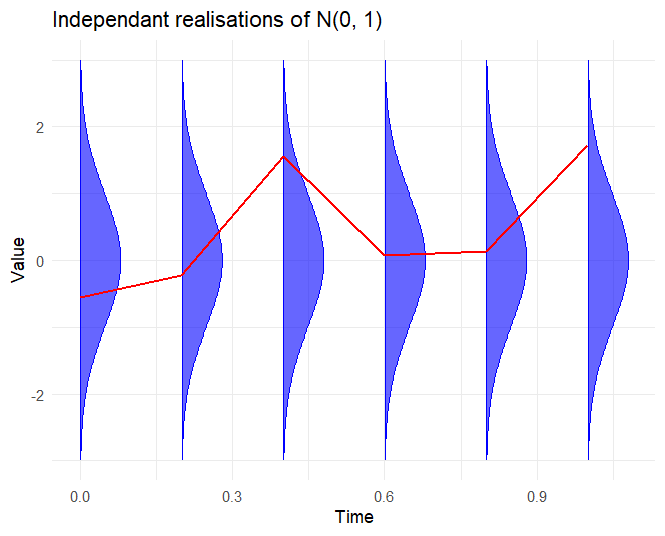
\includegraphics[width=\textwidth]{images/bb_without_cov.png}
    \caption{Folge von unabhängigen Normalverteilten Zufallsvariablen. Die Realisierungen sind chaotisch.}
    \label{fig:bb_without_cov}
  \end{minipage}\hfill
  \begin{minipage}{0.48\textwidth}
    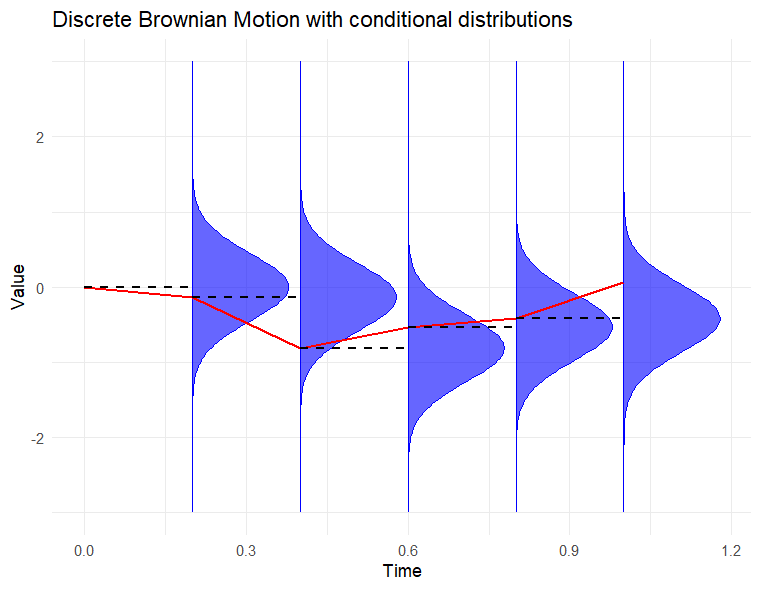
\includegraphics[width=\textwidth]{images/bb_with_cov.png}
    \caption{Visualierung der bedingten Verteilung der diskreten Brownschen Bewegung.}
    \label{fig:bb_with_cov}
  \end{minipage}
\end{figure}
\end{bem}

\begin{korr}[Martingal-Eigenschaft der Brownschen Bewegung]
Die Brownsche Bewegung $W_t$ ist ein Martingal.
\textit{Beweis.} Aus der bedingten Verteilung folgt
$$
E(W_t | W_s = v) = v.
$$
Damit ist $W_t$ ein Martingal. \qed
\end{korr}  

\begin{satz}[Stetigkeit der Pfade]
Der Pfad $t \mapsto W_t(\omega)$ ist fast sicher stetig.
\textit{Beweis.}
Für den Beweis wird eine neue Funktionen-Folge $\hat W_t^{(n)}(\omega), n \in \Bbb N$
definiert, wobei $\hat W_t^{(n)}(\omega)$ die lineare Interpolation der Werte $W_{k/2^n}(\omega), k=0,1,2,\ldots$ ist. 
Ohne Beschränkung der Allgemeinheit wird das Intervall $[0,1]$ betrachtet. Für $n \in \Bbb N$ und $k=0,\dots,2^n-1$ setze
$$I_{n,k}:=\big[k2^{-n},(k+1)2^{-n}\big].$$
Da die $I_{n,k}$ eine Zerlegung von $[0,1]$ bilden, ist
$$
\begin{aligned}
M_n &:=\sup_{t\in[0,1]}\big|\hat W^{(n+1)}_t-\hat W^{(n)}_t\big| 
\\ &= \max_{0\le k<2^n} \sup_{t\in I_{n,k}} \big|\hat W^{(n+1)}_t-\hat W^{(n)}_t\big| =\max_{0\le k<2^n}|Z_{n,k}|
\end{aligned}
$$
Für die unabhängigen Inkremente $Z_{n,k}$ mit
$$
Z_{n,k}\sim N\!\big(0,2^{-(n+2)}\big).
$$
Für eine Normalverteilung $Z\sim \mathcal N(0,\sigma^2)$ und jedes $\varepsilon>0$ gilt (siehe z. B. Boucheron 2013 \cite{boucheron_concentration_2013} S. 2)
$$
P(|Z| >\varepsilon) \le 2\exp\!\Big(-\frac{\varepsilon^2}{2\sigma^2}\Big).
$$
Mit der Schranke folgt
$$
P(M_n>\varepsilon) \le \sum_{k=0}^{2^n-1} P(|Z_{n,k}|>\varepsilon)
\le 2^n\cdot 2\exp\!\Big(-\frac{\varepsilon^2}{2\sigma_n^2}\Big)
= 2^{\,n+1}\exp\!\Big(-\frac{\varepsilon^2}{2\sigma_n^2}\Big).
$$
Man wählt nun eine spezifische Folge $\varepsilon_n$ so, dass sich aus der rechten Seite eine geometrische Reihe ergibt. Setze
$$
\varepsilon_n := \sqrt{2(n+1)}\,\sigma_n.
$$
Dann gilt
$$
\frac{\varepsilon_n^2}{2\sigma_n^2}=n+1,
$$
und damit
$$
P(M_n>\varepsilon_n)\le 2^{\,n+1} e^{-(n+1)} = \big(2e^{-1}\big)^{\,n+1}.
$$
Da $2e^{-1}<1$ ist, ist die Folge auf der rechten Seite geometrisch und insbesondere summierbar. Folglich
$$
\sum_{n=1}^\infty P(M_n>\varepsilon_n) < \infty.
$$
Mit dem Reihenkriterium für fast sichere Konvergenz folgt, dass $M_n\to 0$ fast sicher.
Für $m \gt n \ge N$ beliebig gilt
$$\sup_{t}|\hat W^{(m)}_t - \hat W^{(n)}_t| \leq \sum_{k=n}^{m-1} M_k. \underset{N \to \infty} \longrightarrow 0$$
Weil jedes $\big(\hat W^{(n)}\big)_{n\in\Bbb N}$ eine stückweise lineare Funktion ist, folgt
dass $\big(\hat W^{(n)}\big)_{n\in\Bbb N}$ fast sicher eine Cauchy-Folge in $\Vert \cdot \Vert_{\infty}$ ist.
$\big(\hat W^{(n)}\big)_{n\in\Bbb N}$ konvergiert also gleichmäßig gegen den Grenzpfad $\widetilde W$, der stetig ist. \qed

\end{satz}

\newpage